\section{Related work}
\label{sec:relatedwork}

\begin{figure*}[t]
	\centering
	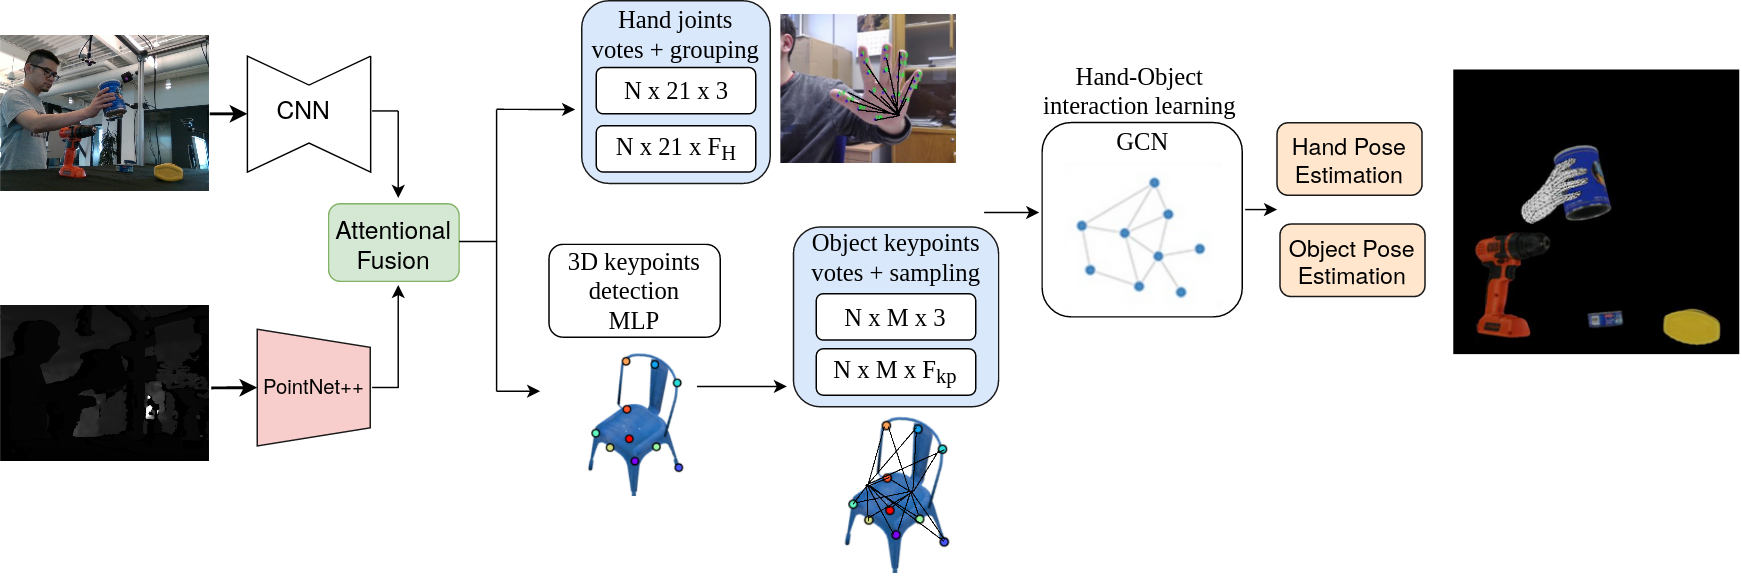
\includegraphics[width=0.95\linewidth]{Figs/Hand-Object_pose.png}
	\caption{\textbf{Overview of our proposal}. Our method takes both color and depth maps as input data. The color features are extracted by a CNN, while the 3D features are calculated by PointNet++ architecture. These two types of features are then fused at a pixel level to obtain the new distinctive features by the adaptive fusion network. This network learns to predict the weight matrix that facilitates beneficial features to eclipse the tedious information. We design a deep Hough voting-based network to vote for 21 MANO hand joints and $M=9$ selected object keypoints. A GCN-based network is deployed to learn the constraints and interdependencies between the hand and object poses to boost the estimation performance.}
	\label{fig:Hand_pose}
\end{figure*}


\subsection{Hand-object pose estimation}
The naive approach for this mission is treating the hand \cite{yang2022dynamic, madadi2017end, deng2017hand3d, oberweger2017deepprior++, iqbal2018hand} and manipulated object \cite{wang2019densefusion, schwarz2015rgb, qi2018frustum, zhou2018voxelnet} separately without considering their interdependence. They underestimate the extraordinary relationship between hand gestures and object shapes. Several approaches overcome this problem by jointly learning the shapes of both hands and objects from RGB images.  \cite{hasson2020leveraging} looks into photometric consistency between neighboring frames to reconstruct hand-object shapes under interactions. \cite{tekin2019h+} handles hand action classification to assist the process of estimating hand-object interactions. \cite{liu2021semi} introduce a semi-supervised learning framework leveraging spatial-temporal consistency to improve estimation performance. However, the absence of depth information makes the process of learning physical constraints and interactions latent. In addition, the transformation from 2D to a 3D world is accurately difficult due to the high degree of nonlinearity. In contrast, some methods solely exploit depth images. \cite{choi2017robust} designs an architecture that firstly predicts hand and object centers and then learns global orientations and hand grasp configurations while interacting with objects. \cite{zhang2021single, goudie20173d} segments 2D hand and object regions from depth images and then optimizes the reconstruction process of interacting motions. This method, however, learns the depth images by a 2D CNN backbone and hence cannot radically observe the geometric information. \cite{oberweger2019generalized} deploys a feedback loop to revise the flawed estimation results using depth images only. RGB-D input, on the other hand, has received relatively less attention due to the puzzle of an effective collaboration of two distinctive input formats still holds a secret. \cite{kyriazis2013physically} focuses on the physical laws of hand actions from RGB-D input to benefit hand-object interaction interpretations. \cite{tsoli2018joint} tracks hands and objects in dealing with a complex scenario in which manipulated objects are deformable. 

\subsection{RGB-D fusion}
With the common of color-depth camera, a wide range of computer vision research such as object segmentation \cite{chen2021global, chen2020bi, park2017rdfnet, zhang2021non} and 6D object detection \cite{wang2019densefusion, tian2020robust, saadi2021optimizing} has been inspired to learn and incorporate color and depth features from RGB-D images. The RGB image and depth image belong to different modalities, so most fusing feature methods are \cite{wang2021brief}: image layer fusion, feature layer fusion, and output layer fusion. While image layer fusion concatenates the input data before feeding to CNNs, feature layer fusion means learning color and depth data in two distinguished architectures but sharing the learning process. Output layer fusion, on the other hand, integrates two feature maps that are separately extracted by two backbone networks. However, fusion RGB-D features for hand-object pose estimation is less attractive because most of the mentioned methods have a mutual weak point which is extracting features from depth maps by 2D CNNs. This makes the 3D spatial feature output latent and oblivious. Motivated by \cite{wang2019densefusion}, we develop a network that not only exports geometric information and geometric constraints by using Pointnet++ \cite{qi2017pointnet++}, but also adaptively and selectively adjusts features at each pixel before fusing to achieve the reliable performance. 

\subsection{Graph convolutional network  for pose estimation}
The power of graph convolutional networks has recently captured the researchers' attention in solving the problem of pose estimation. The network provides the relationship awareness of input data, hence can cope with the problem of a large number of DoF in hand pose estimation. \cite{kong2020sia} allows the network to be spatially aware to boost the 2D hand keypoints prediction. Interm of jointly estimate hand-object pose estimation, \cite{doosti2020hope} develops two graph convolutional network-based architectures for two missions. The first one detects 2D hand joints and 2D object corners, while the second lifts 2D keypoints to 3D coordinates. \cite{almadani2021graph} also designs two steps of firstly predicting 2D hand-object poses. Afterward, this method boosts the performance by gradually providing more information such as the third dimension and mesh vertices to the graph-based network. \cite{tse2022collaborative} proposes attention-guided graph convolution to iteratively share hand and object estimator between two branches for learning the mutual occlusion. This success inspires us to develop a graph-based network for hand-object interaction learning but instead directly feed the 3D features to learn the relationship without the need of lifting 2D information to 3D coordinates, which might cause unpredictable mistakes.
